\documentclass[aspectratio=169,11pt,t]{beamer}
% ============================================================
%  ksa-cs-v2: ksa-cs-lecture-template.tex 스타일 + 한글, v2 덱(16:9)용.
%    - 짙은 네이비 헤드라인 (섹션 이름 + 프레임마다 점)
%    - 꽉 찬 파란 제목 막대, 둥근 그림자 블록
%    - 한글: Noto Sans CJK KR (fontspec)
%  사용:
%    \documentclass[aspectratio=169,11pt,t]{beamer}
%    \input{<..>/theme/ksa-cs-v2.tex}
%  ksa-theme.tex 의 매크로(\kb \kq, ksablue/ksared 등)도 같은 이름으로 둔다
%  -> v2 덱 본문을 거의 그대로 옮길 수 있다.
% ============================================================

\usepackage{fontspec}
\usepackage{amsmath,amssymb}
\usepackage{tikz}
\usepackage{listings}
\usepackage{graphicx}
\usepackage{booktabs}
\usepackage{varwidth}
% enumitem 은 넣지 않는다 (beamer 글머리표가 사라진다)

\defaultfontfeatures{Ligatures=TeX}
\setmainfont{Noto Sans CJK KR}
\setsansfont{Noto Sans CJK KR}
\setmonofont{Noto Sans Mono CJK KR}[Scale=0.92]
\usefonttheme{professionalfonts}

% ---------- 기본 틀 ----------
\usetheme{default}
\useinnertheme[shadow=true]{rounded}
\setbeamertemplate{navigation symbols}{}
\setbeamersize{text margin left=1em,text margin right=1em}

% ---------- 색 (템플릿 원본 값) ----------
\definecolor{navydark}{HTML}{191959}
\definecolor{navydim}{HTML}{8888B0}
\definecolor{navytitle}{HTML}{262686}
\definecolor{navyblue}{HTML}{3333B2}
\definecolor{blockbodybg}{HTML}{E9E9F3}
\definecolor{examplegreen}{HTML}{006000}
\definecolor{examplebg}{HTML}{E5EFE5}
\definecolor{alertred}{HTML}{BF0000}
\definecolor{alertbg}{HTML}{F9E5E5}
% ksa-theme.tex 와 같은 이름 (본문 호환)
\colorlet{ksablue}{navytitle}
\colorlet{ksabluedk}{navydark}
\definecolor{ksagold}{HTML}{D6CBB1}
\definecolor{ksagolddk}{HTML}{A9976B}
\colorlet{ksared}{alertred}
\definecolor{ksagray}{HTML}{5B5B5B}

\setbeamercolor{structure}{fg=navyblue}
\setbeamercolor{alerted text}{fg=alertred}
\setbeamercolor{frametitle}{bg=navytitle,fg=white}
\setbeamercolor{title}{fg=white,bg=navytitle}
\setbeamercolor{block title}{bg=navytitle,fg=white}
\setbeamercolor{block body}{bg=blockbodybg,fg=black}
\setbeamercolor{block title example}{bg=examplegreen,fg=white}
\setbeamercolor{block body example}{bg=examplebg,fg=black}
\setbeamercolor{block title alerted}{bg=alertred,fg=white}
\setbeamercolor{block body alerted}{bg=alertbg,fg=black}
\setbeamercolor{item}{fg=navyblue}
\setbeamertemplate{itemize item}[circle]
\setbeamertemplate{itemize subitem}[triangle]

% ---------- 헤드라인: miniframes (섹션 이름 + 점) ----------
\useoutertheme[subsection=false]{miniframes}
\setbeamerfont{section in head/foot}{size=\tiny}
\setbeamercolor{section in head/foot}{bg=navydark,fg=white}
\setbeamercolor{mini frame}{fg=white}
\setbeamertemplate{mini frames}[circle]

% ---------- 제목 막대: 폭 꽉 채움, 두 줄까지 ----------
\setbeamerfont{frametitle}{size=\normalsize,series=\bfseries}
\setbeamertemplate{frametitle}{%
  \nointerlineskip
  \begin{beamercolorbox}[wd=\paperwidth,ht=2.7ex,dp=1.1ex,leftskip=.3cm,rightskip=.3cm]{frametitle}%
    \usebeamerfont{frametitle}\insertframetitle
  \end{beamercolorbox}}

% ---------- 쪽 번호: 오른쪽 아래 ----------
\setbeamertemplate{footline}{%
  \hfill
  {\color{navydim}\scriptsize\insertframenumber\,/\,\inserttotalframenumber}%
  \hspace{3mm}\vspace{2mm}%
}

% ---------- 표지: 템플릿처럼 헤드라인은 그대로, 가운데 둥근 그림자 상자에 제목 한 줄 ----------
% 덱에서:  {\setbeamertemplate{footline}{}\begin{frame}[c,noframenumbering]\titlepage\end{frame}}
\setbeamercolor{title}{fg=white,bg=navyblue}
\makeatletter
\setbeamertemplate{title page}{%
  \vfill
  \centering
  \begin{minipage}{0.84\paperwidth}
  \begin{beamercolorbox}[wd=\linewidth,sep=7pt,center,rounded=true,shadow=true]{title}
    {\usebeamerfont{title}\inserttitle\par}%
    \ifx\insertsubtitle\@empty\else\vskip0.4em{\usebeamerfont{subtitle}\insertsubtitle\par}\fi
  \end{beamercolorbox}
  \end{minipage}\par\vskip1.6em
  {\usebeamerfont{author}\color{navytitle}\insertauthor\par}\vskip0.3em
  {\usebeamerfont{institute}\color{ksagray}\insertinstitute\par}
  \vfill
}
\makeatother
\setbeamerfont{title}{series=\bfseries,size=\Large}
\setbeamerfont{subtitle}{size=\normalsize}
\setbeamerfont{author}{size=\normalsize}
\setbeamerfont{institute}{size=\small}

% ksa-theme 호환: 덱이 \renewcommand{\ksacredit}{..} 를 해도 되게 (꼬리말에는 안 쓴다)
\newcommand{\ksacredit}{}

% ---------- 강조 ----------
\newcommand{\hl}[1]{\textcolor{alertred}{#1}}
\newcommand{\hlb}[1]{\textcolor{navyblue}{#1}}
\newcommand{\kb}[1]{\textbf{\color{ksablue}#1}}
\newcommand{\kq}[1]{\textbf{\color{ksared}#1}}

% ---------- 파이썬 코드 (템플릿과 같은 색) ----------
\definecolor{codekw}{HTML}{0033B3}
\definecolor{codebuiltin}{HTML}{BF0000}
\definecolor{codestr}{HTML}{067D17}
\definecolor{codecomment}{HTML}{8C8C8C}
\definecolor{codenum}{HTML}{1750EB}
\lstdefinestyle{py}{
  language=Python, basicstyle=\ttfamily\scriptsize,
  keywordstyle=\color{codekw}\bfseries, stringstyle=\color{codestr},
  commentstyle=\color{codecomment}\itshape, numberstyle=\color{codenum},
  emph={print,len,range,sum,input,int,str,float,list,dict,append,remove,sorted,abs,min,max},
  emphstyle=\color{codebuiltin}, showstringspaces=false, keepspaces=true,
  columns=fixed, basewidth=0.52em, aboveskip=1mm, belowskip=1mm, xleftmargin=2mm,
  breaklines=true
}
\lstset{style=py}

% 원본 덱 (ksa-theme): slides/v2/ml1/week14/word2vec/ -- 그림은 거기 figs/ 를 그대로 쓴다
\setbeamerfont{author}{size=\normalsize}
\setbeamerfont{institute}{size=\small}
\graphicspath{{../../../v2/ml1/week14/word2vec/figs/}{../../../assets/}}
\makeatletter
\newcommand{\markpage}[1]{\protected@write\@auxout{}{\string\newlabel{#1}{{\the\c@framenumber}{}}}\hypertarget{#1}{}}
\newcommand{\pref}[1]{\hyperlink{#1}{\textcolor{ksagolddk}{(p.\ref{#1})}}}
\makeatother

\renewcommand{\ksacredit}{Machine Learning and Deep Learning \,\textperiodcentered\, word2vec}
\title{word2vec 단어를 벡터로}
\subtitle{함께 나오는 단어를 보면 그 단어를 안다}
\author{Machine Learning and Deep Learning}
\institute{한국과학영재학교 (KSA)}
\date{}
\begin{document}
{\setbeamertemplate{footline}{}\begin{frame}[c,noframenumbering]\titlepage\end{frame}}


\section{질문}
% --- 오늘의 질문
\begin{frame}{오늘의 질문: 왕 $-$ 남자 $+$ 여자 $=$ ?}
\vfill
\centering
{\Huge king $-$ man $+$ woman $=$ \kb{?}}\vskip1.2em
{\large 단어를 숫자 벡터로 바꾸면 \textbf{뜻으로 계산}할 수 있을까?}\\[0.6em]
{\large 원-핫 (단어마다 칸 하나): 모든 단어 사이 거리가 같다}\\[0.2em]{\large 고양이 $\leftrightarrow$ 강아지 $=$ 고양이 $\leftrightarrow$ 자동차}
\vfill
\note{king 빼기 man 더하기 woman은 무엇일까요? 단어를 숫자 벡터로 바꾸면 이런 식으로 뜻을 계산할 수 있을까요? 가장 단순한 방법은 원-핫, 단어마다 칸 하나를 주는 겁니다. 그런데 원-핫 벡터는 모든 단어 사이 거리가 똑같습니다. 고양이와 강아지 사이나 고양이와 자동차 사이나 같죠. 뜻이 비슷한 단어가 가까운 벡터를 만드는 방법, 2013년 구글의 word2vec을 배웁니다.}
\end{frame}

\section{아이디어}
% --- 아이디어
\begin{frame}{비결: 함께 나오는 단어를 보면 그 단어를 안다}
\vfill
\centering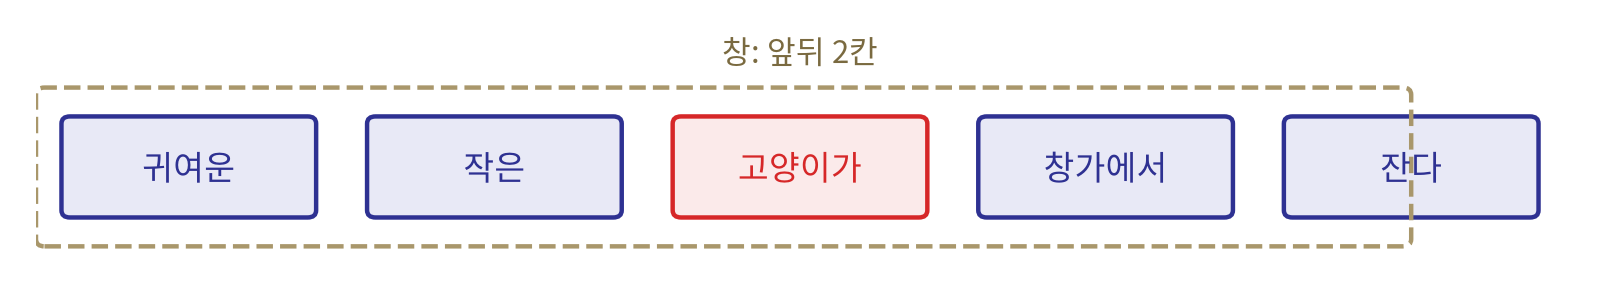
\includegraphics[width=0.78\linewidth]{w2v_window.png}\par\vskip0.4em
{\large ``You shall know a word by the company it keeps'' \quad (Firth, 1957)}\\[0.6em]
{\large 고양이가 자리에 \textbf{강아지가} 와도 주변이 같다 \quad $\to$ 두 단어의 벡터를 가깝게}\\[0.2em]
{\large 사과 · 자동차는 이런 주변에 잘 안 나온다 \quad $\to$ 멀게}
\vfill
\note{비결은 언어학자 퍼스가 1957년에 한 말입니다. 단어는 그 단어와 함께 다니는 단어들로 알 수 있다. 귀여운 작은 고양이가 창가에서 잔다에서, 고양이가의 앞뒤 두 칸, 귀여운, 작은, 창가에서, 잔다가 이웃입니다. 고양이가 자리에 강아지가가 와도 주변 단어는 똑같죠. 그러면 두 단어의 벡터를 가깝게 만들면 됩니다. 사과나 자동차는 이런 주변에 잘 나오지 않으니 멀어집니다.}
\end{frame}

% --- Skip-gram, CBOW
\begin{frame}{두 가지 연습 문제: Skip-gram · CBOW}
\markpage{arch}
\vfill
\centering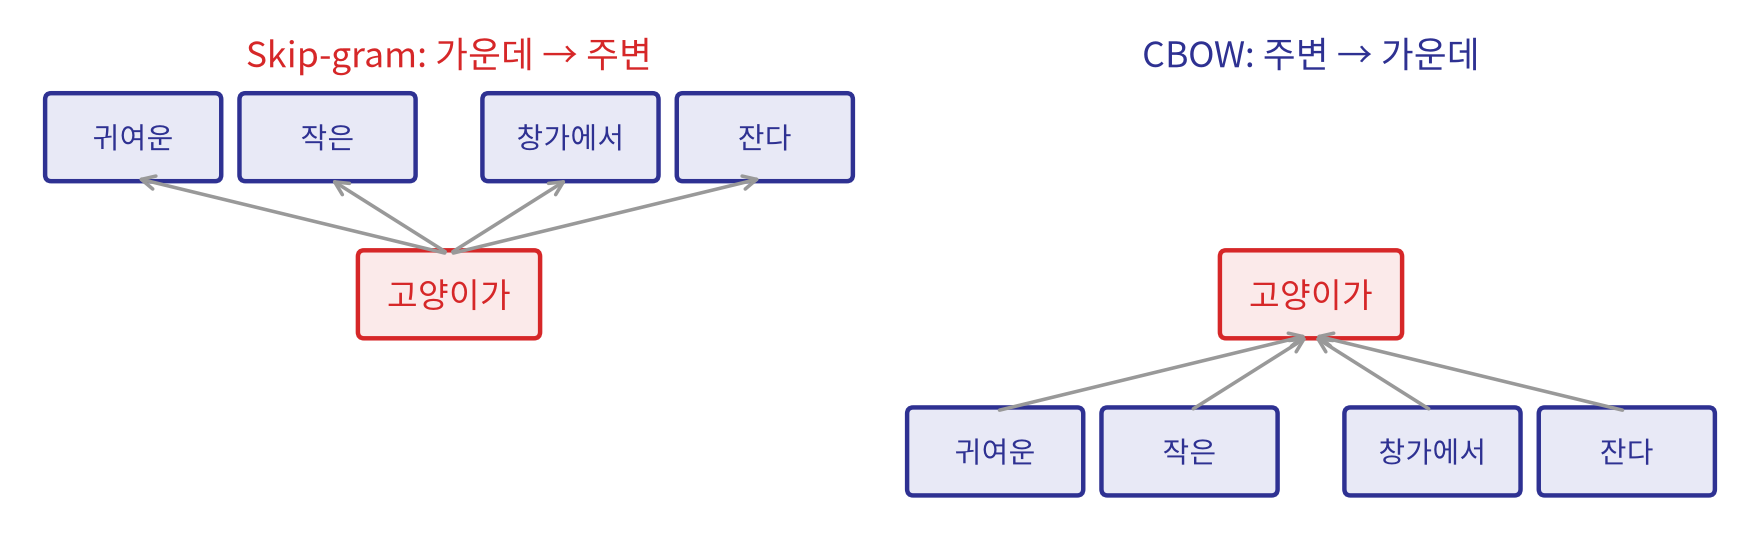
\includegraphics[width=0.86\linewidth]{w2v_arch.png}\par\vskip0.3em
\renewcommand{\arraystretch}{1.3}
{\large\begin{tabular}{lll}
 & Skip-gram & CBOW (Continuous Bag-of-Words)\\\hline
문제 & 가운데 단어로 주변 단어 맞히기 & 주변 단어들 (평균) 로 가운데 맞히기\\
특징 & 느리지만 \textbf{드문 단어}에 강하다 & 빠르고 흔한 단어에 강하다
\end{tabular}}
\vfill
\note{word2vec은 이 생각을 연습 문제 두 가지로 만들었습니다. Skip-gram은 가운데 단어 하나로 주변 단어들을 맞히고, CBOW는 반대로 주변 단어들의 벡터를 평균 내서 가운데 단어를 맞힙니다. 진짜 목적은 문제를 맞히는 게 아니라, 문제를 풀면서 생기는 단어 벡터입니다. Skip-gram은 단어마다 여러 문제가 생겨 느리지만 드문 단어도 잘 배우고, CBOW는 빠르고 흔한 단어에 강합니다. 오늘 실험은 Skip-gram입니다.}
\end{frame}

% --- 식
\begin{frame}{식으로: 함께 나오면 내적을 크게}
\markpage{formula}
\vfill
\centering
{\large 단어마다 벡터 두 개: \quad 가운데일 때 $\mathbf{v}_w$, \quad 주변일 때 $\mathbf{u}_w$ \quad (보통 100 $\sim$ 300칸)}\vskip0.4em
{\LARGE\[ \text{손실} = -\log \sigma(\mathbf{v}_c \cdot \mathbf{u}_o) - \sum_{k=1}^{K} \log \sigma(-\mathbf{v}_c \cdot \mathbf{u}_{n_k}) \]}\vskip0.2em
\renewcommand{\arraystretch}{1.4}
{\large\begin{tabular}{ll}
$c, o$ & 창 안에서 \textbf{실제로} 함께 나온 쌍 $\to$ 내적을 크게\\
$n_1, \dots, n_K$ & 아무렇게나 뽑은 단어 $K$ 개 (네거티브) $\to$ 내적을 작게\\
\end{tabular}}\\[0.4em]
{\small 단어 7만 개 전부에 softmax 를 하는 대신 네거티브 5개만 \quad 흔한 단어 (the, of) 는 솎아 낸다}
\vfill
\note{식으로 보면, 단어마다 벡터가 두 개 있습니다. 가운데에 올 때의 v와 주변에 올 때의 u입니다. 창 안에서 실제로 함께 나온 쌍 c와 o는 내적을 크게, 즉 시그모이드가 1에 가깝게 만들고, 아무렇게나 뽑은 단어 K개, 네거티브 단어와의 내적은 작게 만듭니다. 원래는 다음 단어를 7만 개 단어 전체의 softmax로 맞혀야 하지만, 이렇게 네거티브 5개만 쓰면 계산이 훨씬 빠릅니다. 또 the나 of처럼 너무 흔한 단어는 일부를 솎아 내고 학습합니다.}
\end{frame}

\section{손으로}
% --- 손 계산
\begin{frame}{손으로 한 번}
\vfill
\centering
{\large $\mathbf{v}_{\text{고양이}} = (1, 0, 1)$, \quad 함께 나온 $\mathbf{u}_{\text{잔다}} = (1, 1, 0)$, \quad 네거티브 $\mathbf{u}_{\text{자동차}} = (0, -1, 1)$}\vskip0.6em
\renewcommand{\arraystretch}{1.6}
{\Large\begin{tabular}{lll}
함께 나온 쌍 & $\mathbf{v} \cdot \mathbf{u} = 1$, \ $\sigma(1) = 0.73$ & $-\ln 0.73 = 0.31$\\
네거티브 & $\mathbf{v} \cdot \mathbf{u} = 1$, \ $\sigma(-1) = 0.27$ & $-\ln 0.27 = 1.31$\\\hline
손실 & & \kb{1.63}
\end{tabular}}\vskip0.6em
{\large 기울기: $\mathbf{v}_{\text{고양이}}$ 를 \textcolor{ksablue}{잔다 쪽으로}, \textcolor{ksared}{자동차 반대쪽으로} 조금 옮긴다}
\vfill
\note{3칸짜리 벡터로 계산해 봅시다. 고양이의 v가 1, 0, 1이고, 함께 나온 잔다의 u가 1, 1, 0, 아무렇게나 뽑은 자동차의 u가 0, 마이너스 1, 1입니다. 고양이와 잔다의 내적은 1, 시그모이드 1은 0.73, 마이너스 로그는 0.31입니다. 고양이와 자동차의 내적도 1인데, 네거티브는 마이너스 내적의 시그모이드, 0.27을 쓰니 마이너스 로그가 1.31입니다. 손실은 1.63입니다. 경사 하강을 하면 고양이 벡터는 잔다 쪽으로, 자동차 반대쪽으로 조금씩 옮겨 갑니다. 이걸 수천만 번 하면 비슷한 주변을 가진 단어들이 모입니다.}
\end{frame}

\section{실험}
% --- 실험: 이웃
\begin{frame}{실험: 위키백과 1,700만 단어로 직접 학습}
\markpage{exp}
\vfill
\centering
{\large text8 (영어 위키백과 일부) \quad 단어 7만 개 \quad 100칸 \quad 쌍 5,600만 개 \quad CPU 약 2분}\vskip0.6em
\renewcommand{\arraystretch}{1.3}
{\large\begin{tabular}{ll}
단어 & 가장 가까운 단어 (코사인 유사도)\\\hline
cat & dog 0.71, cats, rabbits, albino, rat\\
computer & computers 0.81, computing, hardware\\
apple & \textbf{macintosh} 0.83, iigs, iic \quad (과일이 아니라 회사)\\
korea & taiwan 0.79, thailand, seoul, china
\end{tabular}}\vskip0.6em
{\large 뜻을 알려 준 적이 없다 \quad 주변 단어만 맞혔을 뿐}
\vfill
\note{직접 학습해 봤습니다. text8이라는 영어 위키백과 일부, 1700만 단어로, 단어 7만 개에 100칸짜리 벡터를 Skip-gram으로 학습했습니다. 함께 나온 쌍이 5600만 개, 노트북 CPU로 약 2분 걸렸습니다. cat과 가장 가까운 단어는 dog, cats, rabbits입니다. computer는 computers, computing, hardware입니다. 재밌는 건 apple인데, 가장 가까운 단어가 macintosh입니다. 위키백과에서는 과일보다 회사 이야기가 많기 때문이죠. 우리는 뜻을 하나도 알려 주지 않고, 주변 단어만 맞혔을 뿐입니다.}
\end{frame}

% --- 비유
\begin{frame}{벡터로 비유 풀기: $b - a + c$ 와 가장 가까운 단어}
\markpage{analogy}
\vfill
\begin{columns}[c]
\column{0.5\linewidth}\centering
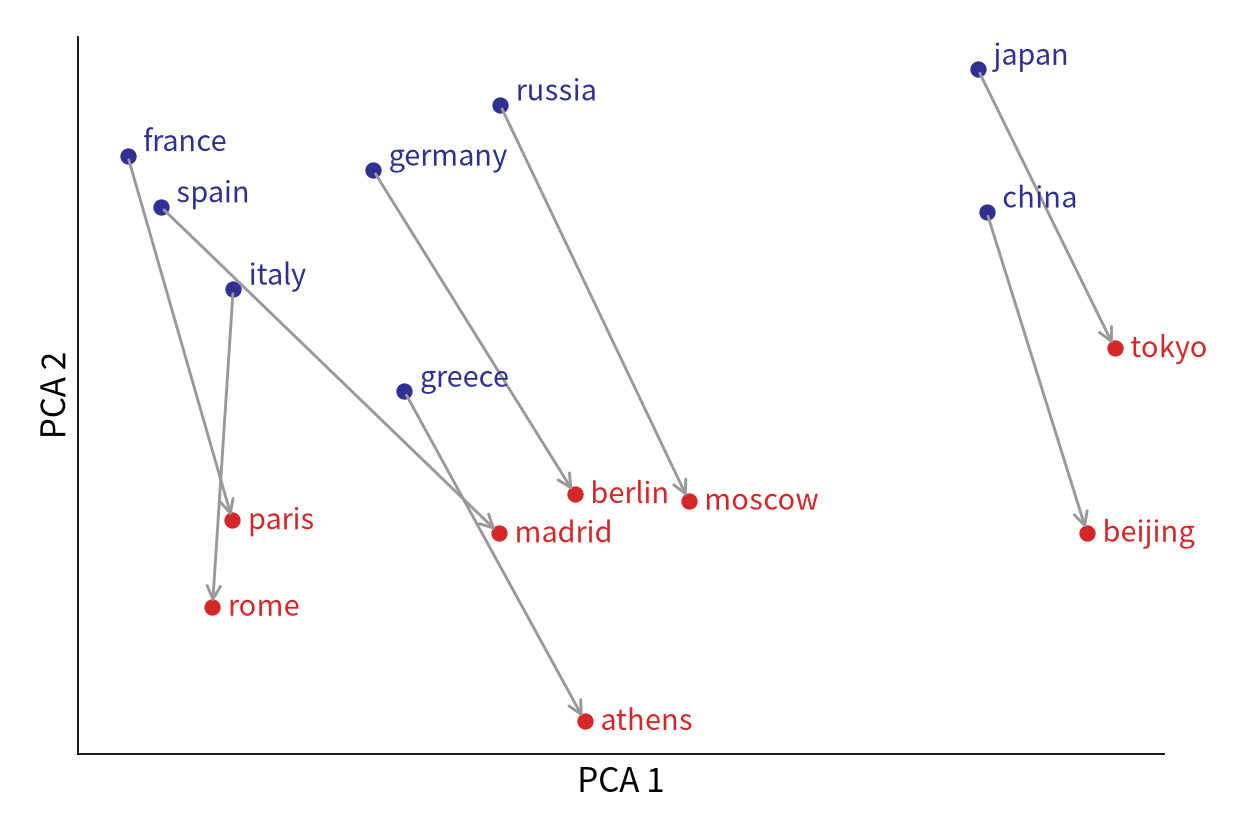
\includegraphics[width=\linewidth]{w2v_capitals.png}\\
{\small 나라 $\to$ 수도 화살표가 거의 나란하다}
\column{0.48\linewidth}
\renewcommand{\arraystretch}{1.3}
{\normalsize\begin{tabular}{ll}
paris $-$ france $+$ germany & \kb{berlin}\\
tokyo $-$ japan $+$ korea & \kb{seoul}\\
he $-$ man $+$ woman & \kb{she}\\
bigger $-$ big $+$ small & \kb{smaller}\\
king $-$ man $+$ woman & \kq{5위}: queen
\end{tabular}}\\[0.5em]
{\small 유명한 king $\to$ queen 은 우리 작은 학습에선 5위 (1위 aquitaine)}
\end{columns}
\vfill
\note{이제 벡터 계산으로 비유를 풀어 봅니다. paris 빼기 france 더하기 germany와 가장 가까운 단어는 berlin, tokyo 빼기 japan 더하기 korea는 seoul입니다. he 빼기 man 더하기 woman은 she, bigger 빼기 big 더하기 small은 smaller입니다. 왼쪽 그림처럼 나라에서 수도로 가는 화살표가 거의 나란하기 때문입니다. 그런데 유명한 king 빼기 man 더하기 woman은 우리 학습에서는 queen이 5위였습니다. 1위는 프랑스 지역 이름 aquitaine이었습니다. 왕 이야기에 자주 나오는 단어들이죠. 논문은 단어 수십억 개로 학습했고, 우리는 1700만 개라 이런 차이가 납니다. 유명한 예라고 늘 1위로 나오는 건 아닙니다.}
\end{frame}

% --- 비유 시험
\begin{frame}{Google 비유 문제로 채점}
\vfill
\centering
{\large Mikolov 외 (2013) 의 비유 문제 \kb{19,544}개 \quad (예: Athens : Greece = Baghdad : ?)}\vskip0.6em
\renewcommand{\arraystretch}{1.4}
{\large\begin{tabular}{lccc}
 & 문제 & 3만 단어 안에 있는 것 & 1위로 맞힘\\\hline
의미 (수도, 통화, 가족 $\cdots$) & 8,869 & 4,103 & \kb{23.3\%}\\
문법 (비교급, 과거형, 복수 $\cdots$) & 10,675 & 8,165 & \kb{29.1\%}
\end{tabular}}\vskip0.8em
{\large 3만 개 단어 중 정확히 1위여야 정답 \quad 찍으면 0.003\%}\\[0.2em]
{\small 데이터를 늘리고 (Google News 약 1,000억 단어), 벡터를 키우면 (300칸) 훨씬 높아진다}
\vfill
\note{논문에는 비유 문제 19544개가 있습니다. 아테네와 그리스의 관계가 바그다드와 무엇의 관계와 같은지 같은 문제입니다. 우리 벡터는 자주 나온 3만 단어만 저장했으니, 네 단어가 다 들어 있는 문제만 풀었습니다. 수도, 통화, 가족 같은 의미 문제는 23.3퍼센트, 비교급, 과거형, 복수 같은 문법 문제는 29.1퍼센트를 1위로 맞혔습니다. 낮아 보이지만 3만 개 단어 중 정확히 1위여야 하니, 찍으면 0.003퍼센트입니다. 구글이 공개한 벡터는 뉴스 약 1000억 단어로 300칸 벡터를 학습해서 훨씬 높습니다.}
\end{frame}

% --- 한계와 다음
\begin{frame}{한계와 다음 걸음}
\vfill
\centering
\renewcommand{\arraystretch}{1.6}
{\large\begin{tabular}{ll}
단어마다 벡터 \textbf{하나} & ``apple'' 은 회사든 과일이든 같은 벡터\\
& ``bank'' 는 은행 · 강둑이 섞인다\\
편향도 배운다 & 글에 있는 성별 · 직업 고정관념이 벡터에 (Bolukbasi 외 2016)\\
문장 전체 & 단어 벡터를 평균 내면 순서를 잃는다
\end{tabular}}\vskip0.8em
{\large $\to$ 문맥에 따라 벡터가 달라지는 \textbf{BERT} (2018) \quad 다음: 임베딩, BERT}
\vfill
\note{word2vec의 한계도 있습니다. 단어마다 벡터가 하나뿐이라, apple은 회사든 과일이든 같은 벡터, bank는 은행과 강둑의 뜻이 섞입니다. 또 글에 있는 성별이나 직업 고정관념도 그대로 배웁니다. 2016년 연구는 man과 computer programmer의 관계가 woman과 homemaker의 관계와 같다고 나오는 걸 보였습니다. 문장 전체를 나타내려고 단어 벡터를 평균 내면 순서도 잃습니다. 이걸 넘어 문맥에 따라 같은 단어도 다른 벡터를 갖는 게 2018년 BERT입니다.}
\end{frame}

\section{연습}
% --- 문제풀이
\begin{frame}{문제풀이}
\vfill
\begin{enumerate}
\item 창이 앞뒤 2칸이면, 5단어 문장 ``귀여운 작은 고양이가 창가에서 잔다'' 에서 (가운데, 주변) 쌍은 몇 개?\vskip0.8em
\item 손 계산에서 $\mathbf{u}_{\text{잔다}}$ 가 $(2, 0, 2)$ 였다면 첫 항 $-\ln \sigma(\mathbf{v} \cdot \mathbf{u})$ 는? ($\sigma(4) \approx 0.982$)\vskip0.8em
\item 단어 7만 개, 100칸이면 학습하는 숫자는 모두 몇 개? (벡터 두 벌)\vskip0.8em
\item 원-핫 벡터로는 king $-$ man $+$ woman 계산이 왜 쓸모없을까?
\end{enumerate}
\vfill
\note{1번 답. 귀여운은 주변 2개, 작은은 3개, 고양이가는 4개, 창가에서 3개, 잔다 2개, 모두 14쌍입니다. 2번 답. 내적이 4, 시그모이드가 0.982, 마이너스 로그는 약 0.018입니다. 3번 답. 7만 곱하기 100 곱하기 2, 1400만 개입니다. 4번 답. 원-핫은 모든 단어가 서로 수직이라, king 빼기 man 더하기 woman이 어느 단어와도 비슷하지 않고, 결과에 가장 가까운 단어는 그냥 king이나 woman 자신입니다.}
\end{frame}

% --- 실습
\begin{frame}{실습}
\vfill
\centering\begin{tabular}{rl}
\large 1 & 창에서 (가운데, 주변) 쌍 만들기, 손 계산 손실 1.63\\[0.5em]
\large 2 & PyTorch 로 Skip-gram + 네거티브 샘플링 직접 학습 (text8 일부)\\[0.5em]
\large 3 & 가까운 단어 · 비유 풀기 (paris $-$ france $+$ germany)
\end{tabular}\vskip1em
text8 (Matt Mahoney, 영어 위키백과 일부) \\[0.4em]\href{https://colab.research.google.com/github/SuminHan/book-ml/blob/main/slides/v2/ml1/week14/word2vec/lab/word2vec.ipynb}{\textcolor{ksagolddk}{▶ Colab에서 실습 노트북 열기}}
\vfill
\note{실습은 세 부분입니다. 첫째, 창에서 가운데와 주변 쌍을 만들고 손 계산 손실 1.63을 확인합니다. 둘째, PyTorch로 Skip-gram과 네거티브 샘플링을 직접 구현해 text8 일부로 학습합니다. 셋째, 가까운 단어를 찾고 비유를 풀어 봅니다.}
\end{frame}

\section{정리}
% --- 정리
\begin{frame}{정리}
\vfill
\centering\large\begin{tabular}{l}
\textbf{word2vec}: 함께 나오는 단어를 맞히는 연습으로 단어 벡터를 배운다 (2013)\\[0.5em]
Skip-gram (가운데 $\to$ 주변) · CBOW (주변 $\to$ 가운데) \quad 네거티브 샘플링\\[0.5em]
1,700만 단어 · 2분: cat $\to$ dog, paris $-$ france $+$ germany $=$ berlin\\[0.5em]
비유 문제 의미 23\% · 문법 29\% \quad 한계: 단어마다 벡터 하나 $\to$ BERT
\end{tabular}
\vfill
\note{정리합니다. word2vec은 함께 나오는 단어를 맞히는 연습으로 단어 벡터를 배웁니다. 가운데로 주변을 맞히는 Skip-gram, 주변으로 가운데를 맞히는 CBOW가 있고, 네거티브 샘플링으로 빠르게 학습합니다. 1700만 단어로 2분 학습해도 cat 옆에 dog가 오고, paris 빼기 france 더하기 germany는 berlin이었습니다. 비유 문제는 의미 23퍼센트, 문법 29퍼센트를 맞혔습니다. 단어마다 벡터가 하나뿐이라는 한계는 BERT로 이어집니다.}
\end{frame}
\end{document}
